\documentclass[12pt]{scrreprt}
%\usepackage{times}
\usepackage{newtxmath,newtxtext}
\usepackage[table]{xcolor}
\definecolor{linkovi}{RGB}{153,182,226}
\definecolor{podnaslovi}{HTML}{3b3d3f}
\usepackage[compact]{titlesec}
\let\oldtextbf\textbf\renewcommand{\textbf}[1]{\textcolor{podnaslovi}{\oldtextbf{#1}}}
\setkomafont{chapter}{\normalfont\Huge\rmfamily\bfseries\color{linkovi}}
\addtokomafont{section}{\normalfont\LARGE\rmfamily\bfseries\color{linkovi}}
\addtokomafont{subsection}{\normalfont\Large\rmfamily\bfseries\color{linkovi}}
\addtokomafont{subsubsection}{\normalfont\large\rmfamily\bfseries\color{linkovi}}

\renewcommand*{\chapterheadstartvskip}{\vspace*{1cm}}
\renewcommand*{\chapterheadendvskip}{\vspace{0.5cm}}
\titlespacing*{\section}{0pt}{10pt}{20pt}
%ovdje možeš mijenjati margine dokumenta
\usepackage[top=2cm, bottom=2cm, outer=2cm, inner=2cm]{geometry}

%bez ovoga newpage i clearpage ne bi radili kako treba
\usepackage{underscore}

%ovo je potrebno za linkove (dolje imaš setup gdje možeš mijenjati boju i još neke stvari)
\usepackage[bookmarks=true]{hyperref}

%sljedeća 3 su vezana za jezik dokumenta
\usepackage[T1]{fontenc} 
\usepackage[utf8]{inputenc}
\usepackage[english]{babel}

%vezani za font
%\usepackage{lmodern}
%\usepackage{tgbonum}

%pozadina (dolje ima background setup gdje se podešava pozadina, slika pozadine neka bude u istom folderu kao i tex file) 
\usepackage[pages=some]{background}

%koristi se za imenovanje slike
\usepackage{caption}

%kako bi podnaslovi mogli ići dalje od 3(koje je default)
\setcounter{secnumdepth}{5}

%za slike
\usepackage{graphicx}

%putanja do slike
\graphicspath{{Images/}}

%za podešavanje pozadine
\backgroundsetup{
	firstpage=true,
	scale=1,
	color=black,
	opacity=0.6,
	angle=0,
	contents={%
		
\includegraphics[width=\paperwidth,height=\paperheight]{12}
	}%
}

%za podešavanje linkova
\hypersetup{
    bookmarks=false,    % show bookmarks bar?
    pdftitle={Software Requirement Specification},    % title
    colorlinks=true,       % false: boxed links; true: colored links
    linkcolor=linkovi,       % color of internal links
    citecolor=black,       % color of links to bibliography
    filecolor=black,        % color of file links
    urlcolor=linkovi,        % color of external links
    linktoc=page            % only page is linked
}
%oboje za linkove
\urlstyle{same}
\usepackage{hyperref}

%bez ovoga javlja grešku kod justify
\usepackage{ragged2e}

%ovo mi je trebalo kako bih izbjegla pagebreak na nekim mjestima, ni sama ne znam kako tačno funkcioniše, samo sam kopirala i radi :D
\newenvironment{absolutelynopagebreak}
{\par\nobreak\vfil\penalty0\vfilneg
	\vtop\bgroup}
{\par\xdef\tpd{\the\prevdepth}\egroup
	\prevdepth=\tpd}

%ovo mijenja "Contents u "Sadržaj"
\addto\captionsenglish{% Replace "english" with the language you use
	\renewcommand{\contentsname}%
	{Sadržaj}%
}

\setlength{\arrayrulewidth}{0.5mm}
%odavde počinje dokument, ovo ranije su samo paketi koji ti trebaju u toku pisanja
\begin{document}
	\begin{titlepage}
		\begin{center}
			\vspace*{10cm}
			\huge{\bfseries{USER INTERFACE SPECIFICATION}}\\
			[2mm]
			\textsc{\LARGE Image Filter App}\\
			[2mm]
			\textsc{\Large April, 2018.}\\
			[3cm]
		\end{center}
		\begin{flushleft}
			\textsc{Grafički dizajner: Alić Amera}
		\end{flushleft}
	\end{titlepage}

\tableofcontents  %sadržaj

\chapter{Forma za početni izgled aplikacije}

\begin{figure}[h]
	\begin{Center}
		
\includegraphics{image2}
	\end{Center}
\end{figure}

\begin{itemize}
	\item Forma se prikazuje dok se aplikacija učitava, što traje par sekundi
\end{itemize}

\chapter{Forma za učitavanje slike}

\begin{figure}[h]
	\begin{Center}
		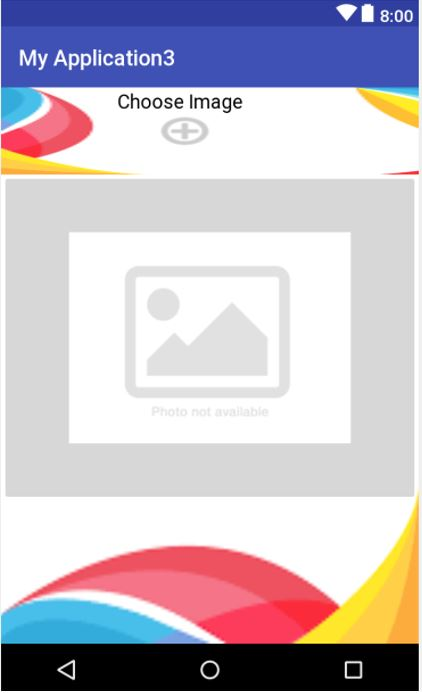
\includegraphics{image3}
	\end{Center}
\end{figure}

\begin{itemize}
	\item Forma se prikazuje odmah nakon što se aplikacija učitala, što traje nekoliko sekundi
	\item Da bi prozor, namijenjen za prikaz slike, učitao sliku neophodno je kliknuti na dugme „Choose Image“ kako bi se odabrala slika koju želimo učitati
\end{itemize}

\section{Forma za odabir slike}

\begin{figure}[h]
	\begin{Center}
		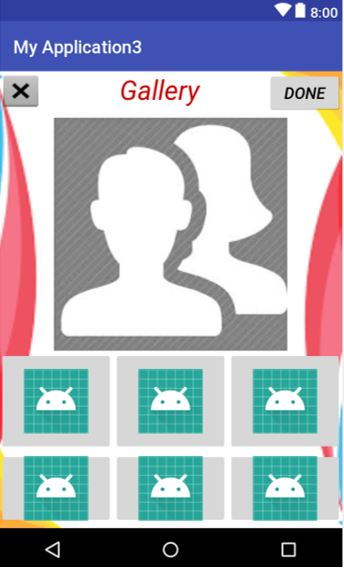
\includegraphics{image4}
	\end{Center}
\end{figure}

\begin{itemize}
 \item	Nakon što smo prethodno kliknuli na dugme „Choose Image“ otvara nam se ova forma za izbor slike
\item	Slike koje su tabelarno prikazane su učitane iz galerije iz memorije uređaja
\item	Pritiskom na svaku sliku ona se pojavljuje u prvom redu u većem formatu
\item	Dugme „X“ nas vraća na prehodnu formu
\item	Dugme „Done“ učitava odabranu sliku u prostor za sliku sa prethodne forme
\end{itemize}

\chapter{Forma za prikaz menija sa dostupnim alatima}

\begin{figure}[h]
	\begin{Center}
		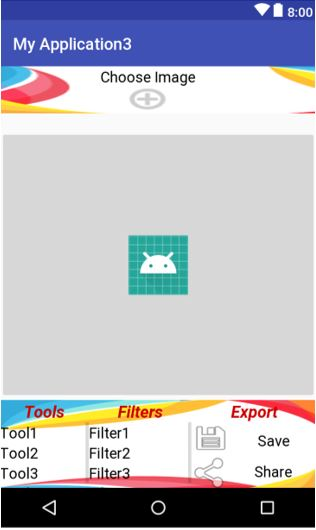
\includegraphics{image5}
	\end{Center}
\end{figure}

\begin{itemize}
	\item Nakon što smo odabrali sliku i kliknuli na dugme „Done“, slika se učitala u prostor za sliku i prikazao se meni, na dnu forme
	\item Meni se sastoji od tri taba: Alati, Filteri i Eksport
	\item Klikom na neki fileter iz taba „Filters“ otvara se nova forma za uređivanje slike
	\item Klikom na „Save“ otvara se forma za spašavanje slike
	\item Klikom na dugme „Share“ otvara se forma za dijeljenje slike na društvenim mrežama
\end{itemize}
\break
\section{Forma za prikaz uređivanja slike}

\begin{figure}[h]
	\begin{Center}
		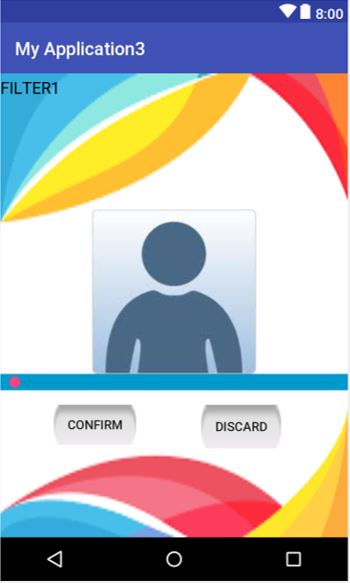
\includegraphics{image6}
	\end{Center}
\end{figure}

\begin{itemize}
	\item	Nakon što smo kliknuli na „Filter1“ prikazuje se forma za uređivanje slike
	\item	Forma sadrži sliku koju želimo urediti kao i „seekbar“ namijenjen za podešavanje količine ili intenziteta primjenjenog filtera na slici
	\item	Dugme „Confirm“ primjenjuje filter na sliku i učitava je u prostor za sliku u formi za prikaz slike
	\item	Dugme „Discard“ omogućava odbacivanje primjenjenog filtera i vraćanje na prethodni meni
\end{itemize}

\chapter{Forma za nakon uređivanja}

\begin{figure}[h]
	\begin{Center}
		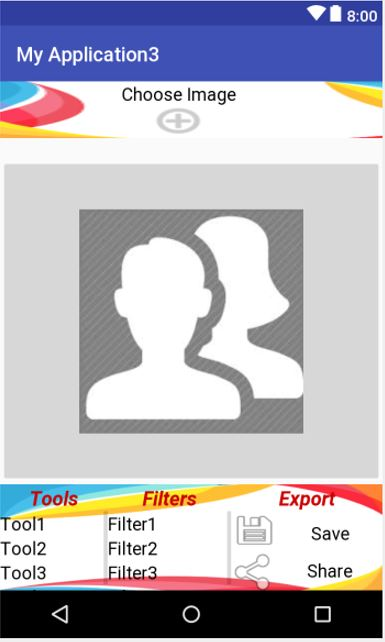
\includegraphics{image7}
	\end{Center}
\end{figure}

\begin{itemize}
	\item Prikaz forme nakon uređivanja slike
\end{itemize}

\break
\section{Forma za pohranjivanje slike}

\begin{figure}[h]
	\begin{Center}
		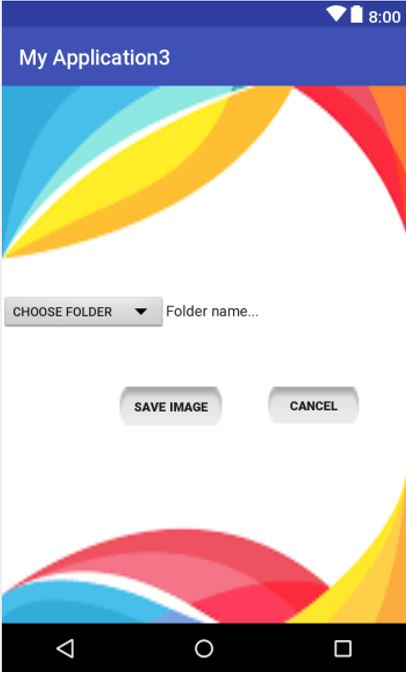
\includegraphics{image8}
	\end{Center}
\end{figure}

\begin{itemize}
	\item	Forma se otvara nakon što smo kliknuli na dugme „Save“ u formi za prikaz slike
	\item	Dugme „Choose folder“ omogućava da pristupimo folderima mobilnog uređaja i da izaberemo gdje želimo spasiti sliku
	\item  „Edit text: Folder name“ omogućava da se odmah navede folder u koji se želi spasiti slika
	\item  Dugme „Save Image“ spašava sliku u izabrani folder, u slučaju da on postoji
	\item  Dugme „Cancel“ nas vraća na prethodnu formu, što je forma za prikaz slike
\end{itemize}
\break
\section{Forma za dijeljenje slike na društvenim mrežama}

\begin{figure}[h]
	\begin{Center}
		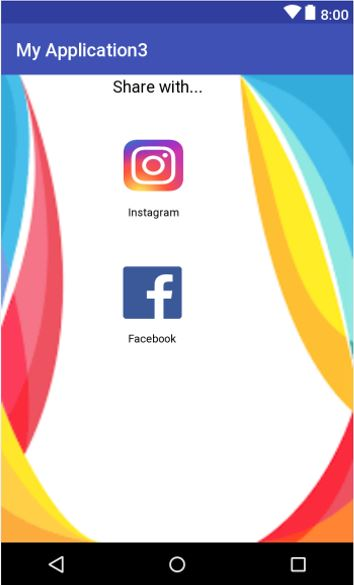
\includegraphics{image9}
	\end{Center}
\end{figure}

\begin{itemize}
	\item	Forma se otvara nakon što se klikne na dugme „Share“ na formi za prikaz slike
	\item	Dugme sa ikonom društvene mreže "Instagram" omogućava pristup Instagramu te objavu slike na toj društvenoj mreži
	\item  Dugme sa ikonom društvene mreže "Facebook" omogućava pristup Instagramu te objavu slike na toj društvenoj mreži
\end{itemize}
\end{document}
